\documentclass[11pt,dvipdfmx,cjk]{beamer}
% パッケージの追加
\usepackage{graphicx} % 図を表示するためのパッケージの追加
\usepackage{bm} % 太字イタリックを使えるようにする 

% beamer に関する設定
% Adobe Reader の文字化けを防ぐおまじない
\AtBeginDvi{\special{pdf:tounicode EUC-UCS2}}
%テーマの指定
\usetheme{Singapore}
\renewcommand{\kanjifamilydefault}{\gtdefault} % 日本語をゴシック体にする
%\mathversion{bold} % これを指定するとデフォルトの数式が太字になる
%\usefonttheme{structurebold}

%--- colorblock 環境の定義
\setbeamercolor{upcolor}{fg=black,bg=blue!40} % ヘッダー部の色指定
\setbeamercolor{lowcolor}{fg=black,bg=blue!20} % body部の色指定
\setbeamertemplate{navigation symbols}{} % 右下に出てくるナビゲーションシンボルを消し飛ばす
\newenvironment{colorblock}%
{\begin{beamerboxesrounded}[upper=upcolor,lower=lowcolor,shadow=true]}%
{\end{beamerboxesrounded}}%

%itemizeの設定
%\setbeamertemplate{itemize item}{\normalsize\raise1.0pt\hbox{$\bullet$}}
%\setbeamertemplate{itemize subitem}{\normalsize\raise1.0pt\hbox{$\blacktriangleright$}}
%\setbeamertemplate{itemize subsubitem}{\normalsize\raise1.0pt\hbox{$\bigstar$}}
\setbeamertemplate{itemize item}{\normalsize\raise0.5pt\hbox{$\bullet$}}
\setbeamertemplate{itemize subitem}{\normalsize\raise1.0pt\hbox{$\blacktriangleright$}}
\setbeamertemplate{itemize subsubitem}{\normalsize\raise1.5pt\hbox{$\bigstar$}}
\renewcommand{\baselinestretch}{1.1}  % 行間設定

% 本文のタイトルなど
\title{Artificial Bee Colonyアルゴリズムによる\\サポートベクトルマシン
のハイパーパラメータ最適化}
\author{2131007 安達 拓真}
\institute{千葉工業大学 情報科学部 情報工学科 4年 山口研究室}
\date{2024年9月3日}


\begin{document} % ここから本文

% タイトルページ表示
\section{タイトル}
\begin{frame}
\maketitle
\end{frame}

\section{既存手法} % セクションを入れると PDF に反映される
\begin{frame}
\frametitle{サポートベクトルマシン(SVM)}
\begin{itemize}
    \item 1995年にC.Cortesらが提案した機械学習アルゴリズム\footnote{ Cortes, C. and Vapnik, V. Support-vector networks, Ma-chine Learning, Vol.20, No.3, pp.273-297, 1995.}
    \item カーネルトリックを使用して、非線形データを高次元空間に写像し、線形分離可能にする 
    \item データを分類する最適な境界線(超平面)を探す                
  \end{itemize}
  \begin{figure}
    \centering
    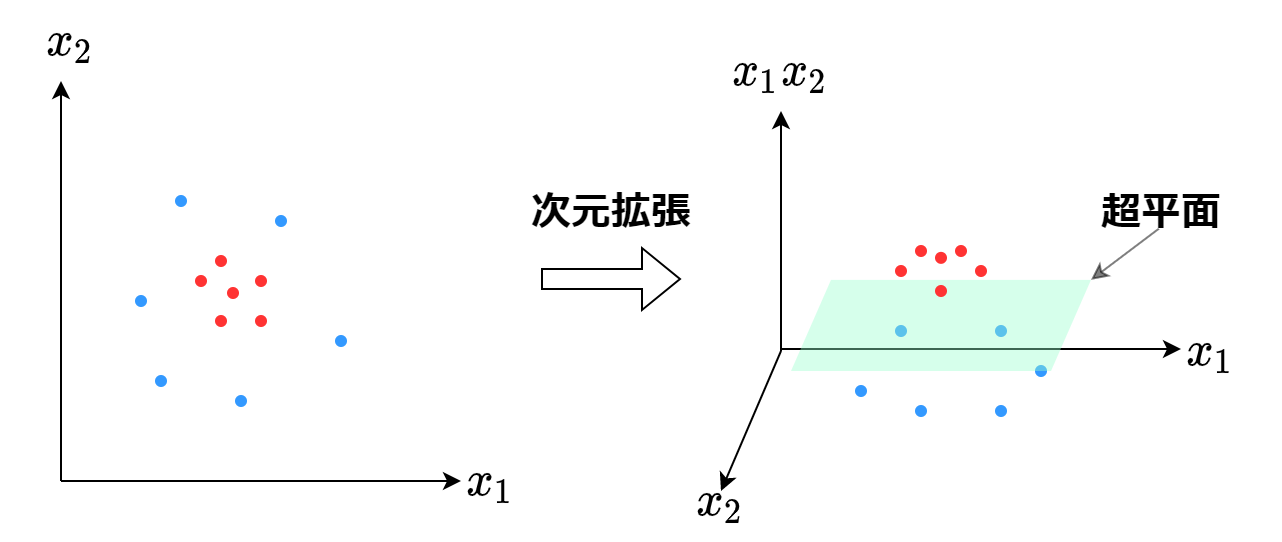
\includegraphics[width=0.8\linewidth]{syazou.png}
   \end{figure}
\end{frame}


%   \frametitle{ハイパーパラメータ最適化(HPO)}
 %   \begin{itemize}
  %    \item 機械学習の性能を最大限に発揮するには適切な\\ハイパーパラメータの設定が必要不可欠
  %    \item 手動では経験的に決めることが多く時間のかかる作業
  %     \begin{itemize}
  %       \item 自動で調節する研究が行われている
   %    \end{itemize}
   %   \item 一般的に計算量が大きいため効率的な探索が必要
   %   \item 離散値、連続値、カテゴリ変数など様々な値を扱う必要がある
   % \end{itemize}
  %\end{frame}
  \begin{frame}
    \frametitle{Artificial Bee Colony(ABC)アルゴリズム}
    \begin{itemize}
      \item 蜂の採餌行動に着目した最適化アルゴリズム\footnote{Karaboga, Dervis. An idea based on honey bee swarm for numerical optimization. Vol. 200. Technical report-tr06, Erciyes university, engineering faculty, computer engineering department, 2005.}
      \item 働き蜂、追従蜂、偵察蜂の三種類の蜂によって各食物源の探索を行い、最適解を求める
      %\item 連続値の最適化を前提としている
      \item ABC自体の設定パラメータは少ない
    \end{itemize}
  \end{frame}
  \begin{frame}
    \frametitle{先行研究\footnote{近藤 久,浅沼 由馬“人工蜂コロニーアルゴリズムによるランダムフォレストとサポートベクトルマシン
    のハイパーパラメータ最適化と特徴選択”,人工知能学会論文誌, vol34-2, pp.1-11, 2019.}におけるSVMのハイパーパラメータ最適化}
    \begin{itemize}
      \item ABCアルゴリズムを使用
      \item カーネル関数をガウスカーネルに固定
      \item 最適化したハイパーパラメータ
      \begin{itemize}
        \item SVMの$C$
        \item ガウスカーネルの$\gamma$
      \end{itemize}
      %式書いたほうがいいかも
    \end{itemize}
\end{frame}
  \section{問題点}
  \begin{frame}
    \frametitle{問題点}
    \begin{itemize}
      \item カーネル関数をガウスカーネルに固定している
      \begin{itemize}
       \item SVMにはガウスカーネル以外にも様々なカーネル関数が適用できる      
      \item カーネル関数によってハイパーパラメータが異なる
    \end{itemize}
    \item ハイパーパラメータ空間の探索範囲が限定的
  \end{itemize}
\end{frame}
  
  \section{提案手法}
  \begin{frame}
    \frametitle{提案手法}
    \begin{itemize}
      \item 4つのカーネル関数とそのハイパーパラメータも最適化対象とする
      \item ABCアルゴリズムにおける解表現は以下のようにする
      \begin{align*}
        \text{解表現:(カーネル関数, C, gamma, coef0, degree)}
      \end{align*}
      \item gamma, coef0, degreeの3つはカーネル関数がもつハイパーパラメータであり
      カーネル関数によって取捨選択する 
      \item カーネル関数の更新はランダムに選ばれた個体とのルーレット選択  
    \end{itemize}
    \begin{align*}
      P = \frac{f(x_j)}{f(x_i)+f(x_j)}  
      \end{align*}
      \begin{align*}
      \text{$i$:更新個体~~$j$:ランダムに選ばれた値}
    \end{align*}
\end{frame}
  
  \end{document}